\documentclass[aspectratio=169]{beamer}

\definecolor{theme}{HTML}{b01419}
\definecolor{accent}{HTML}{0059b3}
\definecolor{offblack}{HTML}{231f20}
\definecolor{link}{HTML}{176ECC}
\definecolor{green}{HTML}{33CC33}
\definecolor{msu}{HTML}{18453B}
\definecolor{duke}{HTML}{001A57}
\setbeamercolor{normal text}{fg=offblack}

\usecolortheme[named=theme]{structure}
\usecolortheme{rose}
\usecolortheme{dolphin}

\makeatletter
\setbeamertemplate{frametitle}{
  \ifbeamercolorempty[bg]{frametitle}{}{\nointerlineskip}%
  \@tempdima=\textwidth%
  \advance\@tempdima by\beamer@leftmargin%
  \advance\@tempdima by\beamer@rightmargin%
  \begin{beamercolorbox}[sep=0.3cm, left, wd=\the\@tempdima]{frametitle}
    \usebeamerfont{frametitle}
    \vbox{}\vskip-2ex%
    \if@tempswa\else\csname beamer@fteleft\endcsname\fi%
    \strut\insertframetitle\strut\par%
    {%
      \ifx\insertframesubtitle\@empty%
      \else%
      {\usebeamerfont{framesubtitle}\usebeamercolor[fg]{
        framesubtitle}\insertframesubtitle\strut\par}%
      \fi
    }%
    \vskip.45ex%
    \hrule %height .6pt%
    \vskip-1.45ex%
    \if@tempswa\else\vskip-.3cm\fi%
  \end{beamercolorbox}%
}
\makeatother

% clean up footer
\beamertemplatenavigationsymbolsempty
\setbeamertemplate{footline}[text line]{
  \parbox{\linewidth}{\vspace*{-10pt}
  \raggedleft \color{offblack} 
  \bf J.\ Scott Moreland (Duke)
  \quad \insertframenumber\,/\,\inserttotalframenumber}
}

% inner theme
\useinnertheme{rectangles}
\setbeamertemplate{itemize item}{
  \raise.30ex\hbox{\vrule width .80ex height .80ex}}
\setbeamertemplate{itemize subitem}{
  \raise.35ex\hbox{\vrule width .70ex height .70ex}}

% for backup slides
\usepackage{appendixnumberbeamer}
\renewcommand\appendixname{Backup}

\usepackage{graphicx}
\usepackage[absolute, overlay]{textpos}
\graphicspath{{../plots/}{fig/}}

\usepackage{amsmath}
\usepackage{amssymb}

\usepackage[T1]{fontenc}
\usepackage[default]{lato}

\usepackage{tikz}
\usetikzlibrary{calc}
\usetikzlibrary{positioning}
\usetikzlibrary{overlay-beamer-styles}

\usepackage[absolute]{textpos}

\usepackage{fontawesome}
\usepackage{ulem}
\newcommand{\soutthick}[1]{%
  \renewcommand{\ULthickness}{.8pt}%
  \sout{#1}%
  }

\newcommand{\trento}{T\raisebox{-0.3ex}{R}ENTo}
\newcommand{\T}{\tilde{T}}
\newcommand{\sqrts}{\sqrt{s_{NN}}}
\newcommand{\sigmaf}{\sigma_\text{fluct}}
\newcommand{\X}{\chi_\text{struct}}
\newcommand{\npartons}{n_\text{partons}}
\newcommand{\dmin}{d_\text{min}^3}
\newcommand{\conference}{\scshape Quark Matter \enskip\textbar\enskip Venice, Italy}
\newcommand{\paddedhline}{\noalign{\smallskip}\hline\noalign{\smallskip}}
\newcommand{\boundellipse}[3]% center, x rad, y rad
{(#1) ellipse [x radius=#2, y radius=#3]
}

\title{Estimating nucleon substructure properties in a\\[.2ex]
unified hydrodynamic model of p-Pb and Pb-Pb collisions}
\author[J.\ S.\ Moreland]{\scshape J.\ S.\ Moreland, J.\ E.\ Bernhard \& S.\ A.\ Bass}
\institute[Duke]{\scshape Duke University}
\date{\scshape 14 May 2018}

\begin{document}

\section{Title}

\begin{frame}[b, plain, noframenumbering]
  \centering
  \textcolor{theme}{\Large \inserttitle} \\[3ex]
  \insertauthor \\
  \insertinstitute \\[2ex]
  \conference \\
  \insertdate \\[6ex]
  \includegraphics[height=1.2cm]{qcdlogo}\quad
  
\includegraphics[height=1.2cm]{nersclogo}\\[3ex]
  \footnotetext[1]{\scriptsize This research used resources of the National Energy Research Scientific Computing Center, a DOE Office of Science User Facility supported by the Office of Science of the U.S.\ Department of Energy under Contract No. DE-AC02-05CH11231.}
\end{frame}

\tikzset{
  box/.style={
    align=center,
    inner sep=1ex,
    background default fill=black!10,
    background default text=black!30,
    background fill=theme!10,
    background text=theme,
  }
}

\newcommand{\boxtitle}[1]{\textbf{#1}\\[.5ex]}

\begin{frame}{\scshape Flow in small systems}
  \smallskip
  \begin{columns}[T]
    \begin{column}{.62\textwidth}
      \bigskip
      Important questions:\\
      \begin{itemize}
        \item Is hydro applicable to small collision systems?
        \item If so, can we fit small system collectivity using current hydro models?
      \end{itemize}
      \smallskip
      First question precludes the second, but also more difficult to answer.\\[1ex]
      Let's tackle the second question \textit{assuming} hydrodynamic models make
      sense down to length scales $\Delta x=.2$~fm.\\[1ex]
      Under this assumption, does a unified hydrodynamic description of p+A and A+A data even exist?
    \end{column}
    \begin{column}{.3\textwidth}
      \centering
      \includegraphics[width=\columnwidth]{pbpb_corr2d}\\
      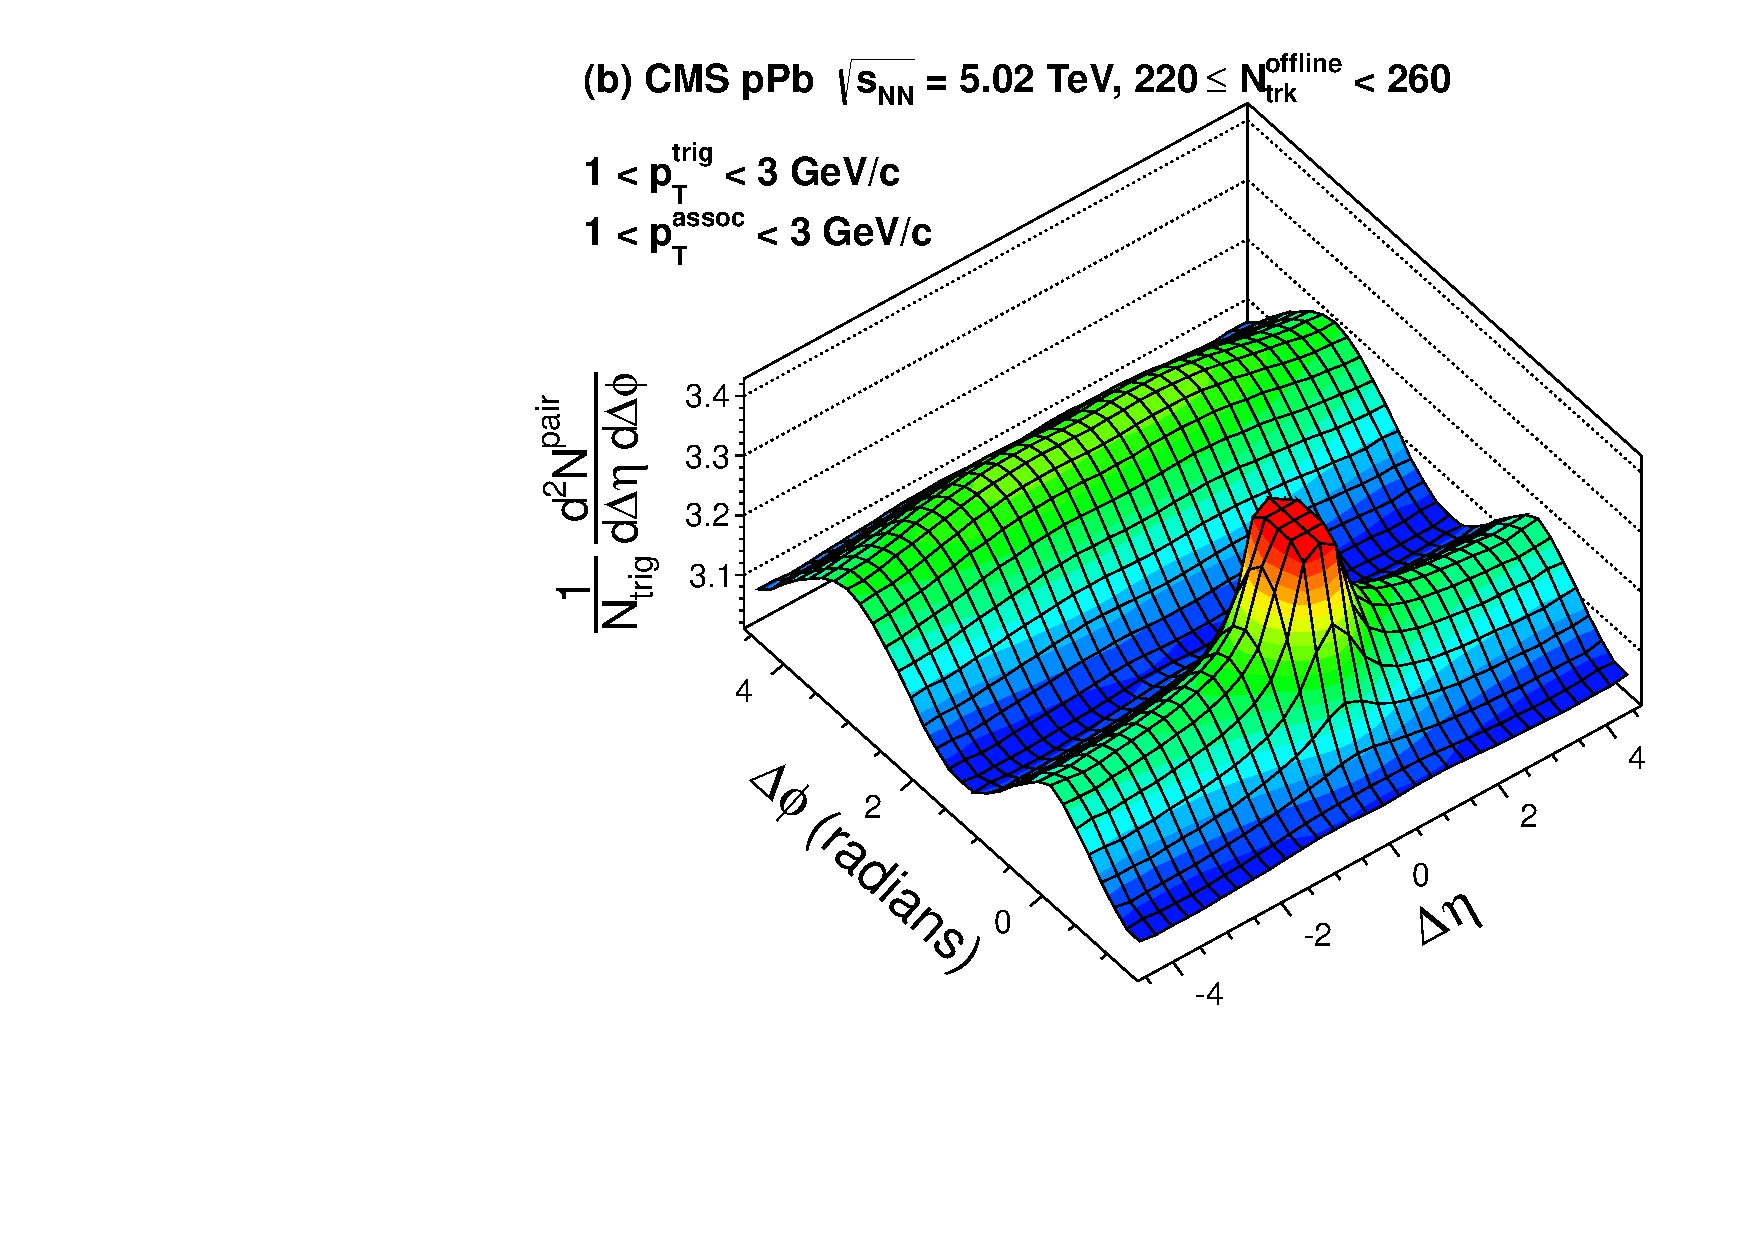
\includegraphics[width=\columnwidth]{ppb_corr2d}
    \end{column}
  \end{columns}

\end{frame}

\begin{frame}[plain, noframenumbering]
  \begin{center}
    \Large I. Bayesian parameter estimation of heavy-ion collisions
  \end{center}
\end{frame}

\begin{frame}[t]{\scshape Heavy-ion collision model}
  \centering
  \medskip
  \begin{tikzpicture}
    \node (a) {\includegraphics[width=.95\textwidth]{hannah_collision}};
    \node[align=left, anchor=north west] at (a.north west) {%
      \scriptsize Figure: H. Petersen, MADAI
      };
  \end{tikzpicture}
  \begin{columns}[T]
    \begin{column}{0.3\textwidth}
      \texttt{\scshape\color{theme} TrENTo} {\small initial conditions}\\
      \smallskip\hrule\medskip
      {\scriptsize parametric entropy deposition}\\
      {\tiny \color{theme}PRC.92.011901}\\[2ex]
      \texttt{\scshape\color{theme} freestream} {\small pre-flow}\\
      \smallskip\hrule\medskip
      {\scriptsize infinitely weak coupling limit}\\
      {\tiny \color{theme} PRC.91.064906, ~PRC.80.034902}
    \end{column}
    \hfill
    \begin{column}{0.3\textwidth}
      \texttt{\scshape\color{theme} VISH2+1} {\small viscous hydro}\\
      \smallskip\hrule\medskip
      {\scriptsize 14-mom.\ approx w/ shear \& bulk}\\
      {\tiny \color{theme} PRC.77.064901, ~J.CPC.2015.08.039}\\[2ex]
      \texttt{\scshape\color{theme}frzout} {\small sampler}\\
      \smallskip\hrule\medskip
      {\scriptsize non-RTA shear \& bulk corrections}\\
      {\tiny\color{theme} J.E.\ Bernhard thesis}
    \end{column}
    \hfill
    \begin{column}{0.3\textwidth}
      \texttt{\scshape\color{theme} UrQMD} {\small Boltzmann cascade}
      \smallskip\hrule\medskip
      {\scriptsize hadronic afterburner, simulate scatterings and decays}\\
      {\tiny\color{theme} PPNP.98.00058, ~JPG.25.9.308}\\[2ex]
      {\scriptsize Final observables calculated as similar as possible to experiment}
    \end{column}
  \end{columns}
  \begin{tikzpicture}[overlay]
    \draw (-3, -.2) -- (-2.7, -.2);
    \draw (-2.7, -.2) -- (-2.7, 3.6);
    \draw (-2.7, 3.6) -- (-2.4, 3.6);
    \draw (2.4, -.2) -- (2.7, -.2);
    \draw (2.7, -.2) -- (2.7, 3.6);
    \draw (2.7, 3.6) -- (3.0, 3.6);
  \end{tikzpicture}
\end{frame}

\begin{frame}[t]{\scshape Bayesian parameter estimation}
  \makebox[\textwidth]{
    \begin{tikzpicture}[overlay]
      \node[box=1, font=\small] (input) at (-5, -1) {
      \boxtitle{Input parameters}
      IC and QGP properties
    };
    \node[box, below=of input.south west, anchor=north west, yshift=.6cm, font=\small] (physics) {
      \boxtitle{Physics theory}
      initial stages, hydro, and\\
      Boltzmann transport
    };
    \node[box, right=of input.east, anchor=west, xshift=-.2cm, font=\small] (model) {
      \boxtitle{Computer model}
      minimum bias event-by-\\
      event simulations
    };
    \node[box, right=of model.east, anchor=west, xshift=-.2cm, font=\small] (gp) {
      \boxtitle{Gaussian process emulator}
      surrogate model
    };
    \node[box, below=of gp.south, anchor=north, font=\small] (mcmc) {
      \boxtitle{MCMC}
      calibrate model to data
    };
    \node[box, below=of mcmc.south, anchor=north, font=\small] (posterior) {
      \boxtitle{Posterior distribution}
      quantitative estimates \\
      of each parameter
    };
    \node[box, left=of mcmc.west, anchor=east, font=\small] (exp) {
      \boxtitle{Experimental data}
      yields, mean $p_T$, flows
    };
    \begin{scope}[color=black!70, ->, thick]
      \draw (input) -- (model);
      \draw ([yshift=-.2cm]physics.north east) -| (model.south);
      \draw (model) -- (gp);
      \draw (gp) -- (mcmc);
      \draw (exp) |- (mcmc);
      \draw (mcmc) -- (posterior);
    \end{scope}
  \end{tikzpicture}
  }
  \begin{textblock}{10}(1, 10)
    {\scshape Objective:}
    \begin{itemize}
        \item Explore parameter space of a given model
        \item Quantify posterior probability of every parameter region
          \textit{given the model, data and \textbf{known uncertainties}}
      \end{itemize}
  \end{textblock}
\end{frame}

\begin{frame}[b, plain]{\scshape Parameter estimates from lead-lead collisions}
  \begin{columns}[b]
    \begin{column}{.43\textwidth}
      \includegraphics<1>[width=\textwidth]{lead_observables_design}
      \includegraphics<2>[width=\textwidth]{lead_observables_posterior}
    \end{column}
    \begin{column}{.57\textwidth}
      \begin{itemize}
        \item Combined analysis of 2.76 and 5.02
          TeV beam energies \textcolor{theme}{\scshape (New!)} 
        \item Parametric initial conditions and medium parameters\
        \item Quantitative estimates on $\eta/s$ and $\zeta/s$ with meaningful uncertainties
        \item See thesis by Jonah Bernhard {\small [\url{99999}]}
      \end{itemize}
      \bigskip
      \includegraphics<1>[width=\textwidth]{region_shear_bulk}
      \includegraphics<2>[width=\textwidth]{region_shear_bulk}
    \end{column}
  \end{columns}
  \medskip
\end{frame}

\begin{frame}[plain, noframenumbering]
  \begin{center}
    \Large II. Adding nucleon substructure to the model
  \end{center}
\end{frame}

\begin{frame}[t]{\scshape Nuclear structure}
  \begin{columns}[T]
    \begin{column}{.4\textwidth}
      \begin{figure}
        \includegraphics[width=.9\columnwidth]{pb208}\\
        Pb$^{208}$ nucleus
      \end{figure}
    \end{column}
    \begin{column}{.6\textwidth}
      \bigskip
      \textcolor{theme}{Original \trento\ model:}
      \begin{itemize}
        \item Sample nucleon radii from spherical or deformed Woods-Saxon distributions
        \item Euler angles resampled to preserve minimum nucleon distance
          $d_\mathrm{min}$ [fm]
        \item Gaussian nucleons of width $w$ [fm]
      \end{itemize}
      \medskip
      \textcolor{theme}{This work:}
      \begin{itemize}
        \item Trade Gaussian nucleon for lumpy nucleon
      \end{itemize}
      \begin{tikzpicture}[absolute, overlay]
        \node (a) at (2, -.75) {\includegraphics[scale=.5]{proton}};
        \node[right=of a.east] (b) {\includegraphics[scale=.5]{proton_partons}};
        \draw[->, thick] (a) -- (b);
      \end{tikzpicture}
    \end{column}
  \end{columns}
\end{frame}

\begin{frame}[t, plain]{\scshape Nucleon substructure}
  \vspace{2em}
  \begin{columns}[t]
    \begin{column}{.2\textwidth}
      \centering \small Sampling radius
      \begin{figure}
        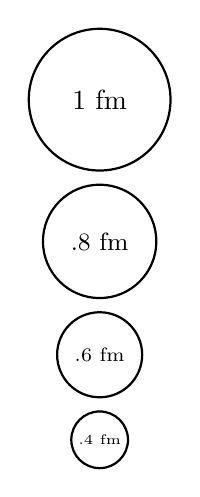
\begin{tikzpicture}[scale=.9]
          \draw[thick] (0,0) circle [radius= 1cm] node (A) {\normalsize 1 fm};
          \draw[thick] (0,-2) circle [radius=.8cm] node (B) {\small .8 fm};
          \draw[thick] (0,-3.6) circle [radius=.6cm] node (C) {\scriptsize .6 fm};
          \draw [thick] (0,-4.8) circle [radius=.4cm] node (D) {\tiny .4 fm};
        \end{tikzpicture}
      \end{figure}
    \end{column}
    \begin{column}{.2\textwidth}
      \centering \small Parton width
      \begin{figure}
        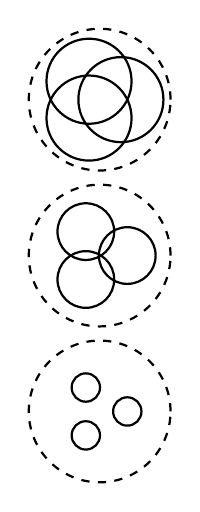
\begin{tikzpicture}[scale=.9]
          \draw [thick, dashed] (0, 0) circle (1cm);
          \foreach \theta in {0, 120, 240}{
            \draw [thick] ({\theta}:.3) circle (.6cm);
          }
          \draw [thick, dashed] (0, -2.2) circle (1cm);
          \foreach \theta in {0, 120, 240}{
            \draw [thick] ({\theta}:.39) [yshift=-2.2cm] circle (.4cm);
          }
          \draw [thick, dashed] (0, -4.4) circle (1cm);
          \foreach \theta in {0, 120, 240}{
            \draw [thick] ({\theta}:.39) [yshift=-4.4cm] circle (.2cm);
          }
        \end{tikzpicture}
      \end{figure}
    \end{column}
    \begin{column}{.2\textwidth}
      \centering \small Parton number
      \begin{figure}
        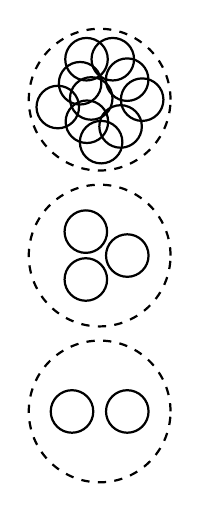
\begin{tikzpicture}[scale=.9]
          \draw [thick, dashed] (0,0) circle (1cm);
          \foreach \theta/\radius in {
            36/0.48, 72/0.6, 108/0.6, 140/0.36, 172/0.12,
            190/0.6, 240/0.36, 272/0.6, 308/0.48, 360/0.6
          }{
            \draw [thick] ({\theta}:\radius) circle (.3cm);
          }
          \draw [thick, dashed] (0, -2.2) circle (1cm);
          \foreach \theta in {0, 120, 240}{
            \draw [thick] ({\theta}:.39) [yshift=-2.2cm] circle (.3cm);
          }
          \draw [thick, dashed] (0, -4.4) circle (1cm);
          \foreach \theta in {0, 180}{
            \draw [thick] ({\theta}:.39) [yshift=-4.4cm] circle (.3cm);
          }
        \end{tikzpicture}
      \end{figure}
    \end{column}
    \begin{column}{.4\textwidth}
      \centering
      \textcolor{theme}{Free parameters:}\\[1ex]
      \begin{itemize}
        \small
        \item Width of the Gaussian distribution used to sample
          parton radial coordinates
        \item Number of Gaussian partons inside each nucleon
        \item Width of the Gaussian partons
      \end{itemize}
      \bigskip
      \textcolor{theme}{Absent from this work:}\\[1ex]
      \begin{itemize}
        \small
        \item Parton spatial correlations,\\
          see talk by Alba Soto Ontoso 
      \end{itemize}
    \end{column}
  \end{columns}
\end{frame}

\begin{frame}[t]{\scshape Cross sections}
  \begin{columns}[T]
    \begin{column}{.5\textwidth}
      \begin{figure}
        \includegraphics[width=\textwidth]{trento_model_part}\\
        \small MC-Glauber cross sections\\
        (proton d.o.f. shown)
      \end{figure}
    \end{column}
    \begin{column}{.5\textwidth}
      \centering \bigskip
      \textcolor{theme}{Original \trento\ model:}
      \begin{align*}
        P_\text{coll} &= 1 - \exp[-\sigma_{gg} T_{pp}(b)] \\
        \sigma_\text{nn}^\text{inel} &= \int 2\pi b\, db\, P_\text{coll}(b)
      \end{align*}
      \only<1>{\includegraphics<1>[scale=.8]{collision_profile}}
      \only<2>{
        \textcolor{theme}{This work:}
        \begin{equation*}
          P_\text{coll} \rightarrow 1 - \prod_{i,j=1}^{n_\text{part}}
          [1 - P_\text{coll}(b_{ij})]
        \end{equation*}
        Solve for opacity parameter $\sigma_{gg}$ numerically
      }
    \end{column}
  \end{columns}
\end{frame}

\begin{frame}[t]{\scshape Participant thickness functions}
  \begin{columns}[T]
    \begin{column}{.5\textwidth}
      \begin{figure}
        \includegraphics[width=\textwidth]{trento_model_thickness}
      \end{figure}
    \end{column}
    \begin{column}{.5\textwidth}
      \centering \bigskip
      \textcolor{theme}{Original \trento\ model:}
      \begin{equation*}
        T_\text{nucleus}(x, y) = \sum\limits_{i=1}^{N_\text{part}}
        \gamma_i\, T_\text{proton}(x - x_i, y - y_i)
      \end{equation*}
      {\small Random weight $\gamma_i$ sampled from Gamma distribution with unit mean
      and variance $1/k$.}\\[2ex]
      \textcolor{theme}{This work:}
      \begin{equation*}
        \gamma_i\, T_\text{proton} \rightarrow \sum\limits_{j=1}^{N_\text{parton}}
        \gamma_j\,T_\text{parton} 
      \end{equation*}
    \end{column}
  \end{columns}
\end{frame}

\begin{frame}[t]{\scshape Entropy deposition}
  \begin{columns}[T]
    \begin{column}{.5\textwidth}
      \begin{figure}
        \includegraphics[width=\textwidth]{trento_model_entropy}
      \end{figure}
    \end{column}
    \begin{column}{.5\textwidth}
      \bigskip \centering
      \textcolor{theme}{Generalized Mean Ansatz:}
      \begin{equation*}
        \frac{dS}{d\eta} \propto T_R(T_A, T_B) \equiv
        \left(\frac{T_A^p + T_B^p}{2}\right)^{1/p}
      \end{equation*}
      \begin{equation*}
        T_R =
        \begin{cases}
          \max(T_A, T_B) & p \rightarrow +\infty, \\[.5ex]
          (T_A + T_B)/2 & p = +1, \\[.5ex]
          \sqrt{T_A T_B} & p = 0, \\[.5ex]
          2\, T_A T_B/(T_A + T_B) & p = -1, \\[.5ex]
          \min(T_A, T_B) & p \rightarrow -\infty.
        \end{cases}
      \end{equation*}
      \smallskip
      \begin{center}
        \small $T$ denotes \emph{participant} thickness function
      \end{center}
    \end{column}
  \end{columns}
\end{frame}

\begin{frame}[t]{\scshape Free streaming}
  \begin{columns}[T]
    \begin{column}{.5\textwidth}
      \begin{figure}
        \includegraphics[width=\textwidth]{trento_model_freestream}\\
        \small arrows: fluid velocity\\weighted by energy density
      \end{figure}
    \end{column}
    \begin{column}{.5\textwidth}
      \bigskip \centering
      \textcolor{theme}{Pre-equillibrium phase:}
      \begin{itemize}
        \small
        \item Massless non-interacting parton gas matched to viscous hydrodynamics
          \textcolor{theme}{\scriptsize PRC.91.064906, PRC.80.034902}.
        \item Must reinterpret initial entropy density as initial gluon density,\,
          $dN_g/y \sim dS/dy$
        \item Initialize hydro with non-zero $u^\mu$ and $\pi^{\mu\nu}$
      \end{itemize}
      \medskip
      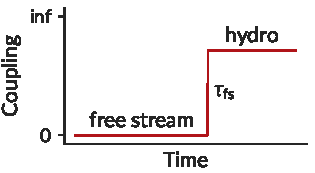
\includegraphics{coupling}
    \end{column}
  \end{columns}
\end{frame}

\begin{frame}[plain, noframenumbering]
  \begin{center}
    \Large III. Simultaneous calibration to\\
    p-Pb and Pb-Pb collisions at $\sqrts=5.02$ TeV
  \end{center}
\end{frame}

\begin{frame}[t]{\scshape Computer experiment design}
  \bigskip
  \begin{columns}[T]
    \begin{column}{.6\textwidth}
      \scriptsize
      \begin{tabular}{lll}
        Parameter         & Description                        & Range           \\
        \paddedhline
        Norm              & Overall normalization              & 12--28          \\
        $p$               & Entropy deposition parameter       & $-1$ to $+1$    \\
        $\sigmaf$         & Relative parton fluct. std.\       & 0--2            \\
        $w$               & Parton sampling radius             & 0.4--1.2 fm     \\
        $\X$              & Parton structure parameter         & 0--1            \\
        $\npartons$       & Number of partons                  & 1--10           \\
        $\dmin$           & Nucleon exclusion volume           & 0--4.9 fm$^3$   \\
        $\tau_{fs}$       & Free streaming time                & 0.1--1.5 fm/$c$ \\
        $\eta/s$ min      & Shear viscosity at $T_c$           & 0--0.2          \\
        $\eta/s$ slope    & Slope above $T_c$                  & 0--8 GeV$^{-1}$ \\
        $\eta/s$ crv      & Curvature above $T_c$              & $-1$ to $1$     \\
        $\zeta/s$ norm    & Bulk viscosity peak height         & 0--0.1          \\
        $\zeta/s$ width   & Bulk viscosity peak width          & 0--0.1 GeV      \\
        $\zeta/s$ temp    & Bulk viscosity peak location       & 150--200 MeV    \\
        $T_\text{switch}$ & Particlization temperature         & 135--165 MeV    \\
      \end{tabular}
    \end{column}
    \begin{column}{.4\textwidth}
      \textcolor{theme}{\scshape Important details:}
      \smallskip
      \begin{itemize}
        \small
        \item Parton width reparametrized:\\[1ex]
          $v = v_\text{min} + \X(v_\text{max} - v_\text{min})$\\[1ex]
          $v_\text{min} = 0.2$~fm,~ $v_\text{max} = w$\\[1ex]
        \item Parton sampling radius is \emph{not} equivalent to the proton radius
          in the proton c.o.m.\ frame, see\\
          \textcolor{theme}{\scriptsize PRC.94.024919}\\[1ex]
        \item Other parameters same as combined Pb+Pb analysis at 2.76 and 5.02 TeV
      \end{itemize}
    \end{column}
  \end{columns}
  \begin{center}
    \color{theme}
    500 design points per collision system, $\mathcal{O}(10^4)$ events per design point!
  \end{center}
\end{frame}

\begin{frame}[plain]
  \begin{tikzpicture}[remember picture, overlay]
    \node[anchor=west] at (current page.west) {
      \includegraphics[height=.95\paperheight]{observables_design}
      };
    \node[anchor=east] at (current page.east) {
      \includegraphics[height=.95\paperheight]{observables_posterior}
      };
    \draw[<-] (current page.center) ++(-.75, 1.7) --
      node[above] {\footnotesize Prior}
      node[below] {\tiny (training data)}
      ++(1.5, 0);
    \draw[->] (current page.center) ++(-.75, -1.2) --
      node[above] {\footnotesize Posterior}
      node[below] {\tiny (samples)}
      ++(1.5, 0);
  \end{tikzpicture}
\end{frame}


\begin{frame}[plain]
  \begin{tikzpicture}
    \node {\includegraphics[height=.98\paperheight]{posterior}};
    \node (title) at (6.0, 3.5) {\color{theme}{\scshape \Large Bayesian posterior}};
    \node<1-2>[draw=none, text width=6.5cm, align=left, below=.2cm of title] (b1) {%
      \small One row (column) for each parameter
      };
    \node<1-2>[draw=none, text width=6.5cm, align=left, below=.1cm of b1] (b2) {%
      \small Diagonal panels: marginal distribution of a single model parameter
      };
    \node<1-2>[draw=none, text width=6.5cm, align=left, below=.1cm of b2] (b3) {%
      \small Off-diagonal panels: joint distribution between a pair of model parameters
      };
    \node<2>[draw=none, text width=6.5cm, align=left, below=.2cm of b3] (b4) {%
      \textcolor{theme}{Let's look at some specific regions...}
      };
    \draw<1-2>[->, thick, theme] (b2.west) to [out=180, in=90] (-.58, 1.3);
    \draw<1-2>[->, thick, theme] (b3.west) to [out=180, in=90] (-.05, 0);
    \node<3>[xshift=-2.8cm, yshift=3.2cm, scale=.3] {
\includegraphics[scale=.15]{magnifying-glass}};
    \node<4>[xshift=-1.2cm, yshift=1.6cm, scale=.3] {
\includegraphics[scale=.15]{magnifying-glass}};
    \node<5>[xshift=-.7cm, yshift=1.1cm, scale=.3] {
\includegraphics[scale=.15]{magnifying-glass}};
  \end{tikzpicture}
\end{frame}

\begin{frame}{\scshape Maximum a posteriori parameters}
  \includegraphics[height=.8\textheight]{find_map}
\end{frame}

\begin{frame}{\scshape Numerical grid error}
  \begin{figure}
    \includegraphics[width=\textwidth]{grid_error}
    \caption{Numerical grid error tame for $dxy=.2 \times \text{parton width}$}
  \end{figure}
\end{frame}

\usebackgroundtemplate{}
\end{document}
